Plan:
\textbf{Two Examples + Algorithm Overview}
\begin{itemize}
\item {Multiple-Path While Loop}
\\
\textbf{The First Challenge/Problem from The Example, 
and the Overview of the New Techniques Targeting This Problem}
\item {Nested While Loop}
\\
\textbf{The Second Challenge/Problem from The Example,
and the Overview of the New Techniques Targeting This Problem}
\end{itemize}
In this section, we discuss two representative examples with
challenges of analyzing the symbolic
\emph{reachability-bound} on
every control location.
We also give the technique overview of our algorithm.
%
\subsection{Multiple-Path Loop}
\label{sec:overview-multiplepath}
\begin{example}[While with Two Paths]
  \label{ex:twoPathsWhile}
  %
  { \small
  \begin{figure}
  \centering
  \begin{subfigure}{.4\textwidth}
    \begin{centering}
    {\small
    $
    \begin{array}{l}
      \kw{twoPathsWhile}(n, m) \triangleq \\
    \clabel{ \assign{i}{n} }^{0} ; \\
    \clabel{ \assign{j}{0} }^{1} ; \\
        \ewhile ~ \clabel{i > 0}^{2} ~ \edo ~ \\
        \qquad \Big(
          \eif(\clabel{j < m}^{3}, \\
          \qquad \qquad \clabel{\assign{j}{j + 1}}^{4}; 
          \clabel{\assign{i}{i - 1}}^{5},\\
          \qquad \qquad \clabel{\assign{j}{0}}^{6});
          \Big)
        \end{array}
        $
    }
    \caption{}
    \end{centering}
    \end{subfigure}
  \begin{subfigure}{.5\textwidth}
    \begin{centering}
  %   \todo{abstract-cfg for two round}
  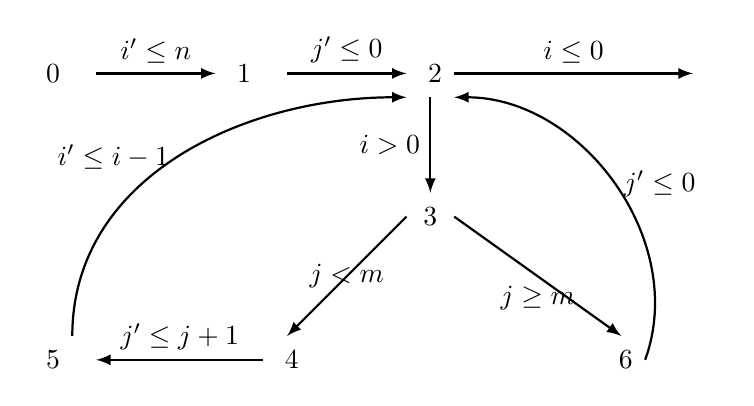
\begin{tikzpicture}[scale=\textwidth/20cm,samples=200]
  \draw[] (-8, 10) circle (0pt) node{{ $0$}};
  \draw[] (-4, 10) circle (0pt) node{{ $1$}};
  \draw[] (0, 10) circle (0pt) node{{ $2$}};
  \draw[] (0, 7) circle (0pt) node{{$3$}};
  \draw[] (-3, 4) circle (0pt) node{{ $4$}};
  \draw[] (-8, 4) circle (0pt) node{{ $5$}};
  \draw[] (4, 4) circle (0pt) node{{ $6$}};
  % Counter Variables
  \draw[] (6, 10) circle (0pt) node {\textbf{$\lex$}};
  % \draw[] (6, 4) circle (0pt) node {{ $ex$}};
  %
  % Control Flow Edges:
  \draw[ thick, -latex] (-7, 10)  -- node [above] {$i' \leq n$}(-4.5, 10);
  \draw[ thick, -latex] (-3, 10)  -- node [above] {$j' \leq 0$}(-0.5, 10);
  \draw[ thick, -latex] (0, 9.5)  -- node [left] {$i > 0$} (0, 7.5) ;
  \draw[ thick, -latex] (0.5, 7)  -- node [below] {$ j \geq m $}  (4, 4.5);
  \draw[ thick, -latex] (-7.5, 4.5)  to  [out=90,in=180]  node [left] {$i' \leq i - 1$ }(-0.5, 9.5);
  \draw[ thick, -latex] (4.5, 4)  to  [out=70,in=0]   node [right] {$j' \leq 0 $}(0.5, 9.5);
  \draw[ thick, -latex]  (-0.5, 7) -- node  {$j < m$}  (-3, 4.5) ;
  \draw[ thick, -latex]  (-3.5, 4) -- node [above] {$j' \leq j + 1$}  (-7, 4) ;
  \draw[ thick, -latex] (0.5, 10)  -- node [above] {$i \leq 0$}  (5.5, 10);
  % \draw[ thick, -latex] (6, 6.5)  -- node [right] {$\top$} (6, 4.5) ;
  \end{tikzpicture}
  \caption{}
    \end{centering}
    \end{subfigure}
  \caption{
  (a) The Two Paths While Loop Example
    (b) The Abstract Execution Control Flow Graph}
      \label{fig:twoPathsWhile}
  \end{figure}
  }
\end{example}

\begin{enumerate}
  \item  \textbf{The Abstract Execution Control Flow Graph} is generated in Figure~\ref{fig:twoPathsWhile}(b).

  \item \textbf{Program Rephrase and Refinement}. 
  \\
  The loop free simple transition paths are computed as follows,
  \[
    \begin{array}{ll}
\tpath_0 = (0 \to 1), (1 \to 2)
&
\tpath_2 = (2 \to 3), (3 \to 6), (6 \to 2)
\\
\tpath_1 = (2 \to 3), (3 \to 4), (4 \to 5), (5 \to 2)
&
\tpath_3 = (2 \to \lex)
\end{array}
\]
\textbf{Refined Program}:
\[
  \tpath_0 ; \rpchoose{2: \rprepeat_2(\rprepeat_1(\tpath_1); \tpath_2) , 
  2: \rprepeat_1(\tpath_1) }; \tpath_3
  \]
  \item \textbf{Ranks}:
  The ranking bounds for every simple transition path:
  \\
  $\absclr(\tpath_0) = 1$ 
  $\absclr(\tpath_1) = n $ \quad
  $\absclr(\tpath_2) = n $ \quad
  $\absclr(\tpath_3) = 1$
  % \\
  % $\bot$ means the algorithm fails in inferring the ranking bound.
    \item \textbf{Outside-In Algorithm} :The \emph{OutIn} bound for the $\rprog$ and every nested repeat patterns.
  \[
    \begin{array}{l}
        \outinB(\tpath_0) = 1
        \\
        \outinB(2: \rprepeat_1(\tpath_1)) = m 
        \\
        \outinB(2: \rprepeat_2(\rprepeat_1(\tpath_1); \tpath_2)) = \lfloor\frac{n}{m}\rfloor
        \\
        \outinB(\rpchoose{\rprepeat_2(\rprepeat_1(\tpath_1); \tpath_2), \rprepeat_1(\tpath_1) })
        = \max\{m, (m  + 1)\times \lfloor\frac{n}{m}\rfloor\}
\end{array}
\]
\item \textbf{Inside-Out Algorithm}
\begin{itemize}
  \item \textbf{Repeat Chain Set}
  \\
  $\rpchset(2, \tpath_1) = \{\rprepeat_1(\tpath_1), \rprepeat_2(\rprepeat_1(\tpath_1); \tpath_2) \to \rprepeat_1(\tpath_1)\}$ \\
  $\rpchset(2, \tpath_2) = \{\rprepeat_2(\rprepeat_1(\tpath_1); \tpath_2) \to \rprepeat_1(\tpath_1)\}$ \\
  $\rpchset(\_, \_) = \emptyset$ 
  % \\
  \item \textbf{Repeat Chain Bound} for every simple transition path $\tpath$ through its \emph{Repeat Chain}s
  \\
  $\rpchB(2, \tpath_1) = \max\{m, m \times \lfloor\frac{n}{m}\rfloor\}$ \\
  $\rpchB(2, \tpath_2) = \lfloor\frac{n}{m}\rfloor$ 
  %
  \item \textbf{Loop Chain}
  \\
  $\lpch(\tpath_0) = \tpath_0$ \qquad
  $\lpch(\tpath_1) = 2\to \tpath_1$ \\
  $\lpch(\tpath_3) = \tpath_3$ \qquad
  $\lpch(\tpath_2) = 2\to \tpath_2$ 
  \item \textbf{{Relative Loop Bound}} for every simple transition path $\tpath$ through its \emph{Loop Chain}
  \\
  $\rpchB(2, \tpath_1) = \max\{m, m \times \lfloor\frac{n}{m}\rfloor\}$ \quad
  $\rpchB(2, \tpath_2) = \lfloor\frac{n}{m}\rfloor$  \\
  $\rpchB(\bot, \tpath_0) = 1$ \quad
  $\rpchB(\bot, \tpath_3) = 1$ 
  \item \textbf{Path-Sensitive Reachability-Bound} for every simple transition path $\tpath$
  \\
  $\inoutB(\tpath_1) = n$ \quad
  $\inoutB(\tpath_2) = \lfloor\frac{n}{m}\rfloor$ \quad
  $\inoutB(\tpath_0) = 1$ \quad
  $\inoutB(\tpath_3) = 1$ 
\end{itemize}
\item \textbf{Path Sensitive Reachability-Bound} on every program control location
\\
$\psRB(\{0, 1, \lex\}) = 1$ \qquad
$\psRB(\{6 \}) = \lfloor\frac{n}{m}\rfloor$ \\
$\psRB(\{4, 5 \}) = \max\{m, m \times \lfloor\frac{n}{m}\rfloor\}$ \quad
$\psRB(\{3, 2 \}) = \max\{m, m \times \lfloor\frac{n}{m}\rfloor\} + \lfloor\frac{n}{m}\rfloor + 1 $ \\
\end{enumerate}
Figure~\ref{fig:whileTwoCounters}(a) shows an example of a two paths loops
with different \emph{reachability-bounds} on the control locations in different paths.
This example is adopted from the example in~\cite{Sumit2010rechability}, which
is a skeleton code from the .Net base-class library.
\\
In this example, given $n \geq m$,
the precise \emph{reachability-bound}s for control locations $4$ and $5$ are both $m \times \lfloor\frac{n}{m}\rfloor$,
for location $2$ and $3$ are $m \times \lfloor\frac{n}{m} + \lfloor\frac{n}{m}\rfloor + 1$, 
and for location $0, 1, \lex$ are $1$.
\\
In order to know that the locations in first branch ($4$ and $5$) are reached at most $m \times \lfloor\frac{n}{m}$ times
while $6$ in second branch $\lfloor\frac{n}{m}\rfloor$ times
 during program execution,
we need to know that the two if branches are interleaved and executed alternatively after each other
during the iterations of the enclosed loop.
\\
However, the method in~\cite{Sumit2010rechability}
can only derive the global loop bound $n + \lfloor\frac{n}{m}\rfloor$
for all three locations $4, 5$ and $6$ because of the path-insensitivity in the method.
To best of my knowledge, there isn't any other work on solving the \emph{reachability-bound} problem.
\\
Among the works on loop bound analysis, \cite{GulwaniJK09} can compute the precise global
loop bound (i.e., $n + \lfloor\frac{n}{m}\rfloor$) for this example path-sensitively.
Using this global bound, we can compute the precise reachability-bound for location $1$ and $2$.
However, the  \emph{reachability-bounds} for control locations $4, 5$ and $6$ are still unclear.
\paragraph{Path-reachability Bound}
The first key idea of this path-sensitive \emph{reachability-bound} analysis algorithm is the \emph{path reachability bound}.
\\
Our algorithm combines the idea of \emph{difference constraint} based program complexity analysis method from \cite{sinn2017complexity}
and the control-flow refinement technique from~\cite{GulwaniJK09} efficiently.
It first
generates the abstract transition graph for the program using the difference constraints, such as Figure~\ref{fig:whileTwoCounters}(b).
Then it transforms every while loop using the control-flow refinement technique from~\cite{GulwaniJK09} and generates a refined program $\rprog$.
% 
The refined program for our $\kw{whileTwoCounters}$ example is
$
  \tpath_0 ; 
  2: \rpchoose{\rprepeat_2(\rprepeat_1(\tpath_1); \tpath_2) , 
  \rprepeat_1(\tpath_1) }; \tpath_3
$, where the simple transition paths $\tpath_0, \cdots$ are as in Figure~\ref{fig:whileTwoCounters}(c).
Every simple path will not interleave with the others. 
Over the refined program, we first compute the \emph{path-reachability bound} for every simple path,
$\inoutB(\rprog, \tpath)$.
It is a bound on the iteration numbers of each simple path.
For this example, the \emph{path-reachability bound} for the three simple transition paths are
$\inoutB(\rprog, \tpath_1) = \max\{m, m \times \lfloor\frac{n}{m}\rfloor\}$ \quad
$\inoutB(\rprog, \tpath_2) = \lfloor\frac{n}{m}\rfloor$ \quad
$\inoutB(\rprog, \tpath_0) = \inoutB(\rprog, \tpath_3) = 1$.
\\
Then we use this bounds
and another \emph{loop-reachability bound}
to compute the \emph{reachability-bound} for each location.
Since there isn't nested loop in this example, we simply sum up the bound of the path where each location shows up
and as its \emph{reachability-bound}, and compute the expected bound for each location.
%
\subsection{Nested Loops with Related Iterator}
\label{sec:overview-nestedwhile}
However, when there exists nested loop, computing the \emph{reachability-bound} for each location encounters another challenge, even though we have
%  local 
iteration bound computed for every path.
Figure~\ref{fig:threeWhile}(a) shows an example of the nested loops with related 
iterators.
This example is adopted from the example in~\cite{GulwaniJK09}, which is common in product code.
\\
In line 8, $i$ is reset by $w$ and $w$ is reset by $j$ at line 5. So the
while $L_6$ is only executed in the first iteration of while loop $L_1$ and $L_3$.
% \\
The while loop $L_3$ at line 3 is executed only in 
the first $m - N$ iterations of the 
$L_1$ because $j$ is reset by $i$ in line 2.
% \\
So the total combined iterations of all the three loops is bounded above by 
$n + m^2 - m \times N$.
And the precise global reachability-bound for location $7$ inside the $L_6$ is $N$,
for locations $4, 5$ and $8$ between the $L_3$ and $L_6$ are $(n-N) \times (m - N)$,
and locations $2$ and $9$ are $n - N$.
\\
\highlight{Notice here the global \emph{reachability-bounds} for the locations inside the loop $L_6$ is 
the same as its loop iteration bound computed by the \emph{path-reachability bound}.
However, for the locations between $L_3$ and $L_6$,
the \emph{reachability-bounds} are the multiplication of the inner and outer loop iteration bounds.}
\\
So far, the loop bound analysis method in \cite{GulwaniJK09} is able to give
an approximation for the $n + (m \times n) + N$. 
The DC-based algorithm in \cite{sinn2017complexity} is able to
compute the precise combined loop bound of $n + m^2 - m \times N$.
\\
But knowing the global loop bound isn't enough to solve the \emph{reachability-bound problem} for locations in nested loops,
especially the locations which are similar to $7$ in $\kw{threeNestedWhile}$ example.
\\
\highlight{
In order to precisely compute how many times the locations inside
$L_6$ is reached globally, we need to know
the numbers of iterations of the outside loop $L_3$ and $L_1$, 
during which the $L_6$ is entered. 
Then we multiply the iteration bounds of the $L_6$ with the number of iterations where it is entered to get the precise
\emph{reachability-bounds} on the control locations inside $L_6$.
This quantity isn't considered or computed in any of the previous works.
}
\\
The \emph{Progress Invariant} method in \cite{GulwaniJK09} is only able to compute
the
%  bound for
%  $L_6$ inside $L_3$ and $L_1$.
bound on iteration numbers
of the inner loop $L_6$ in each iteration of $L_3$ and $L_1$, which are both $N$.
%  the outside loop where it is nested.
% The bound for the iteration numbers $L_6$ in each iteration of $L_3$  and $L_1$ are both $N$, which isn't precise
So they have to over-approximate the reachability-bound for locations inside $L_6$ with the
overall program complexity, i.e., $n + m^2 - m \times N$.
\\
For the same reason, the DC-based algorithm in \cite{sinn2017complexity}
is only able to
compute the precise combined loop bound and the local bound of each loop
separately as well.
We are still unable to know the precise \emph{reachability-bound} for the locations in the innermost loop.
\paragraph*{Loop-reachability Bound.}
The second key idea of our path-sensitive reachability analysis algorithm is the
\emph{loop reachability-bound} for each simple path w.r.t an enclosed loop,
$\lpchB(L:\rprog, \tpath)$.
\highlight{It is a bound on the iterations for
every outside loops w.r.t. the innermost loop where $\tpath$ is enclosed.
Such that during these iterations of each outside loop, the inner loop is entered. 
This is distinguished from the traditional methods, which only compute the bound on the inner loop iterations
in one iteration of the outside loop.}
%
\\
For this example, We first generate its abstract transition graph as well in Figure~\ref{fig:threeWhile}(a),
and then computes its refined program as 
$\rprog = \tpath_0; 1: \rprepeat(\tpath_1;$ 
$3: {\rprepeat(\tpath_2; 6 : {\rprepeat(\tpath_3)}; \tpath_4)}; \tpath_5);$ 
$\tpath_6$,
where the simple paths are shown below the graph in Figure~\ref{fig:threeWhile}(b).
Then in the key step, we compute \emph{loop-reachability bound} for these simple paths w.r.t. each of their nested loops
For example, for $\tpath_3$, we compute
w.r.t. the $L_6$ as
$\lpchB(1: \rprog_1, \tpath_3) = 1$ and
$\lpchB(3: \rprog_3, \tpath_3) = 1$,
where 
$\rprog_1 = {\rprepeat(\tpath_1; 3: {\rprepeat(\tpath_2; 6 : {\rprepeat(\tpath_3)}; \tpath_4)}; \tpath_5)}$
and
$\rprog_3 = {\rprepeat(\tpath_2; 6 : {\rprepeat(\tpath_3)}; \tpath_4)}$.
$\lpchB(3: \rprog_3, \tpath_3) = 1$
means that during all iterations of the loop at $1$, there is only $1$ iteration where the loop at $6$
(the closest loop enclosing $\tpath_3$) is executed.
Among all the other $n - 1$ iterations, the loop $6$ isn't executed at all.
So we compute the \emph{loop-reachability bound}  of the loop $L_3$
w.r.t to this path as $1$.
In the same way, we also compute $\lpchB(1: \rprog_1, \tpath_3) = 1$.
Then we sum up the bound of the path where each location shows up
and as its \emph{reachability-bound} still as before,
and multiply this result by all its \emph{loop-reachability bound}s.
In this way, we compute the accurate reachability bound $N$ for locations inside loop $L_6$.
\begin{example}[Nested Loop with Related Iterators]
  \label{ex:threeNestedWhile}
  %
  %
  { \small
\begin{figure}
\centering
\begin{subfigure}{.4\textwidth}
  \begin{centering}
  {\footnotesize
  $
  \begin{array}{l}
      \kw{relatedNestedWhile}(n, m, N) \triangleq \\
      \clabel{ \assign{i}{0} }^{0} ; \\
          \ewhile ~ \clabel{i < n}^{1} ~ \edo ~ \\
          \qquad \Big(
           \clabel{\assign{j}{m}}^{2} ;\\
           \qquad \ewhile ~ \clabel{j > 0}^{3} ~ \edo ~ \\
           \qquad \qquad \Big(
            \clabel{\assign{j}{j-1}}^{4};
            \clabel{\assign{w}{i}}^{5};\\
            \qquad \qquad \ewhile ~ \clabel{w < N}^{6} ~ \edo ~
            \Big(
              \clabel{\assign{w}{w + 1}}^{7}
                \Big); \\
                \qquad \qquad \clabel{\assign{i}{w}}^{8}
                \Big); \\
                \qquad \clabel{\assign{i}{i+1}}^{9}
            \Big)
      \end{array}
  $
  }
  \caption{}
  \end{centering}
  \end{subfigure}
\begin{subfigure}{.5\textwidth}
  \begin{centering}
%   \todo{abstract-cfg for two round}
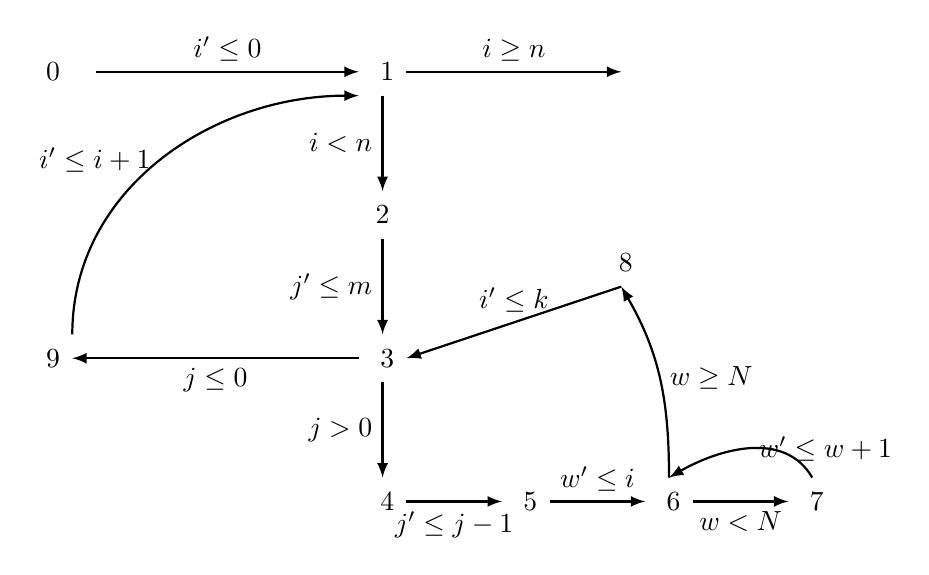
\begin{tikzpicture}[scale=\textwidth/20cm,samples=200]
\draw[] (-7, 10) circle (0pt) node{{ $0$}};
\draw[] (0, 10) circle (0pt) node{{ $1$}};
\draw[] (6, 10) circle (0pt) node {{$\lex$}};
\draw[] (0, 7) circle (0pt) node{{$2$}};
\draw[] (0, 4) circle (0pt) node{{ $3$}};
\draw[] (-7, 4) circle (0pt) node{{ $9$}};
\draw[] (0, 1) circle (0pt) node{{ $4$}};
\draw[] (3, 1) circle (0pt) node{{ $5$}};
\draw[] (6, 1) circle (0pt) node{{ $6$}};
\draw[] (9, 1) circle (0pt) node{{ $7$}};
\draw[] (5, 6) circle (0pt) node{{ $8$}};
% Counter Variables
%
% Control Flow Edges:
\draw[ thick, -latex] (-6, 10)  -- node [above] {$i' \leq 0$}(-0.5, 10);
\draw[ thick, -latex] (0, 9.5)  -- node [left] {$i < n$} (0, 7.5) ;
\draw[ thick, -latex] (0, 6.5)  -- node [left] {$j' \leq m$} (0, 4.5) ;
\draw[ thick, -latex] (0, 3.5)  -- node [left] {$j > 0$} (0, 1.5) ;
\draw[ thick, -latex] (-0.5, 4)  -- node [below] {$j \leq 0$} (-6.5, 4) ;
\draw[ thick, -latex] (-6.5, 4.5)  to  [out=90,in=180]  node [left] {$i' \leq i + 1$ }(-0.5, 9.5);
\draw[ thick, -latex] (0.5, 10)  -- node [above] {$i \geq n$}  (5, 10);
\draw[ thick, -latex] (0.5, 1)  -- node [below] {$j' \leq j - 1$}  (2.5, 1);
\draw[ thick, -latex] (3.5, 1)  -- node [above] {$w' \leq i$}  (5.5, 1);
\draw[ thick, -latex] (6.5, 1)  -- node [below] {$w < N$}  (8.5, 1);
\draw[ thick, -latex] (6, 1.5)  to [out=90,in=-60] node [right] {$w \geq N$}  (5, 5.5);
\draw[ thick, -latex] (9, 1.5)  to  [out=120,in=30] node [right] {$w' \leq w + 1$}  (6, 1.5);
\draw[ thick, -latex] (5, 5.5)  to  node [above] {$i' \leq k$ }(0.5, 4);
\end{tikzpicture}
\caption{}
  \end{centering}
  \end{subfigure}
\caption{
(a) The Example of Nested Loop with Related Iterators
  (b) The Abstract Execution Control Flow Graph}
    \label{fig:threeNestedWhile}
\end{figure}
}
\end{example}

\begin{enumerate}
  \item  \textbf{The Constraint Program (Abstract Control Flow Graph)} is generated in Figure~\ref{fig:threeNestedWhile}(b).

  \item \textbf{Program Refinement}
  \\
  The loop free simple transition paths are computed as follows,
  \[
      \begin{array}{llll}
          \tpath_0 = (0 \to 1)
          &
          \tpath_1 = (1 \to 2), (2 \to 3)
          &           
          \tpath_2 = (3 \to 4), (4 \to 5), (5 \to 6)
          &
          \tpath_3 = (6 \to 7), (7 \to 6)
          \\
          \tpath_6 = (1 \to \lex)
          &
          \tpath_4 = (6 \to 8), (8 \to 3)
          &
          \tpath_5 = (3 \to 9), (9 \to 1)
      \end{array}
      \]
  \textbf{Refined Program}:
  \[
  \rprog = \tpath_0 ; 1: \rprepeat(\tpath_1; 3: \rprepeat(\tpath_2; 6 : \rprepeat(\tpath_3); \tpath_4); \tpath_5); \tpath_6
  \]
  \item \textbf{Outside-In Algorithm} :The \emph{OutIn} bound for the $\rprog$ and every nested repeat patterns.
  \\
$\outinB(\tpath_0) = 1$
\quad
$\outinB(\tpath_6) = 1$
\quad
$\outinB(6 : \rprepeat(\tpath_3)) = N $
\\
$\outinB(3: \rprepeat(\tpath_2; 6 : \rprepeat(\tpath_3); \tpath_4)) = m $
\\
$\outinB(1: \rprepeat(\tpath_1; 3: \rprepeat(\tpath_2; 6 : \rprepeat(\tpath_3); \tpath_4); \tpath_5)) = n - N $
\item \textbf{Inside-Out Algorithm}
\begin{itemize}
  \item \textbf{Repeat Chain Set}
  \\
  $\rpchset(1, \tpath_1) = \{1: \rprepeat(\tpath_1; 3: \rprepeat(\tpath_2; 6 : \rprepeat(\tpath_3); \tpath_4); \tpath_5)\}$
  \\
  $\rpchset(1, \tpath_5) = \{1: \rprepeat(\tpath_1; 3: \rprepeat(\tpath_2; 6 : \rprepeat(\tpath_3); \tpath_4); \tpath_5)\}$
  \\
  $\rpchset(3, \tpath_2) = \{3: \rprepeat(\tpath_2; 6 : \rprepeat(\tpath_3); \tpath_4)\}$
  \\
  $\rpchset(3, \tpath_4) = \{3: \rprepeat(\tpath_2; 6 : \rprepeat(\tpath_3); \tpath_4)\}$
  \\
  $\rpchset(6, \tpath_3) = \{6: \rprepeat(\tpath_3)\}$
  \\
  $\rpchset(_, \_) = \emptyset$ 
  % \\
  \item \textbf{Repeat Chain Bound} for every simple transition path $\tpath$ through its \emph{Repeat Chain}s
  \\
  $\rpchB(1, \tpath_1) = n - N$ \quad
  $\rpchB(1, \tpath_5) = n - N$ \quad
  $\rpchB(3, \tpath_2) = m$ \\
  $\rpchB(3, \tpath_4) = m$ \quad
  $\rpchB(6, \tpath_3) = N$ \quad \quad 
  $\rpchB(_, \_) = \bot $ 
  %
  \item \textbf{Loop Chain}
  \\
  $\lpch(\tpath_1) = 1\to \tpath_1$ \quad
  $\lpch(\tpath_2) = 1 \to 3 \to \tpath_2$ \\
  $\lpch(\tpath_5) = 1\to \tpath_5$ \quad
  $\lpch(\tpath_4) = 1 \to 3 \to \tpath_4$ \\
  \highlight
  {$\lpch(\tpath_3) = 1 \to 3 \to 5 \to \tpath_3$ }\\
  $\lpch(\tpath_0) = \tpath_0$ \quad
  $\lpch(\tpath_6) = \tpath_6$ 
  \item \textbf{{Relative Loop Bound}} for every simple transition path $\tpath$ through its \emph{Loop Chain}
  \\
  $\rpchB(1, \tpath_1) = n - N$ \\
  $\rpchB(1, \tpath_5) = n - N$ \\
  $\rpchB(1, \tpath_2) = n$; \quad $\rpchB(3, \tpath_2) = m$; \\
  $\rpchB(1, \tpath_4) = n$; \quad $\rpchB(3, \tpath_4) = m$ \\
  \highlight{$\rpchB(1, \tpath_3) = 1$; \quad $\rpchB(3, \tpath_3) = 1$; \quad $\rpchB(5, \tpath_3) = N$} \\
  $\rpchB(_, \_) = \bot $ 
  \item \textbf{Path-Sensitive Reachability-Bound} for every simple transition path $\tpath$
  \\
  $\inoutB(\tpath_1) = n - N$ \quad
  $\inoutB(\tpath_2) = n \times m$ \quad
  $\inoutB(\tpath_0) = 1$ 
  \\
  $\inoutB(\tpath_5) = n - N$ \quad
  $\inoutB(\tpath_4) = n \times m$ \quad
  $\inoutB(\tpath_6) = 1$ 
  \\
  $\inoutB(\tpath_3) = N$ \quad
\end{itemize}
\item \textbf{Path Sensitive Reachability-Bound} on every program control location
\\
$\psRB(\{0, \lex\}) = 1$ \quad
$\psRB(\{1\}) = n - N + 1$ \quad
$\psRB(\{2, 9\}) = n - N$ \quad
$\psRB(\{3\}) = n - N + n \times m$ \quad
$\psRB(\{4, 5, 8\}) = n \times m$ \quad
$\psRB(\{7\}) = N$ \quad
$\psRB(\{6\}) = N + n \times m$ 
\end{enumerate}
